% !TeX root = main.tex

\section{The Horn-ICE Learning Framework}
\label{sec:horn-ICE}

The Horn-ICE learning framework~\cite{DBLP:conf/tacas/ChampionC0S18,DBLP:journals/pacmpl/EzudheenND0M18} is a general framework for learning inductive invariants in a black-box setting.
As sketched in Figure~\ref{fig:horn-ice-learning}, this framework consists of two distinct entities---the \emph{learner} and the \emph{teacher}---and proceeds in rounds.
In each round, the learner proposes a candidate invariant $\varphi$ for the program, and the teacher, with access to a verification engine, checks whether the proposed invariant proves the program correct. 
If this is the case, the learning process stops, and the most recent invariant is returned as a proof that the program satisfies its specification.
If, on the other hand, the invariant is not adequate to prove the program correct, the teacher replies with concrete program configurations (so called \emph{counterexamples}), which the learner then uses in the next round to refine its conjecture.
Note that the key feature of this framework is that the learner is completely agnostic of the program and the specification---it is simply constrained to learn some predicate that is consistent with the counterexamples given by the teacher.

\begin{figure}[th]
    \centering
    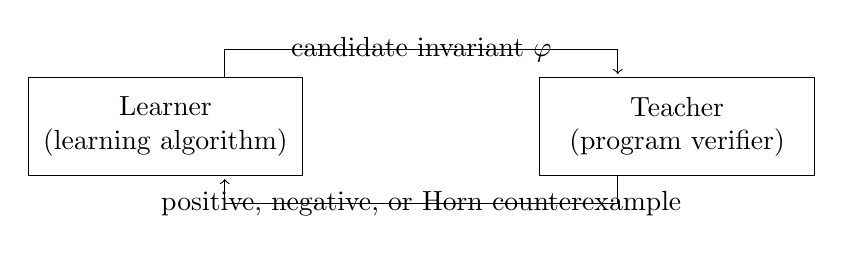
\begin{tikzpicture}
        \node[draw, minimum height=12.5mm, text width=32.5mm, align=center, anchor=east] (learner) at (0, 0) {Learner \\ (learning algorithm)};
        \node[draw, minimum height=12.5mm, text width=32.5mm, align=center, anchor=west] (teacher) at (3, 0) {Teacher \\ (program verifier)};
        
        \begin{scope}[->, shorten >= 1pt]
            \draw (learner.40) -- ++(0, .35) -| node[near start] {candidate invariant $\varphi$} (teacher.140);
            \draw (teacher.220) -- ++(0, -.35) -| node[near start] {positive, negative, or Horn counterexample} (learner.320);
        \end{scope}
    \end{tikzpicture}
    \caption{The Horn-ICE learning framework~\cite{DBLP:conf/tacas/ChampionC0S18,DBLP:journals/pacmpl/EzudheenND0M18}}
    \label{fig:horn-ice-learning}
\end{figure}

To make the Horn-ICE framework mathematically precise, let $P$ be the program under consideration and $\mathcal C$ the set of all program configurations of $P$.
Furthermore, let us fix a finite set $\mathcal P$ of \emph{predicates} $p \colon \mathcal C \to \mathbb B$ over the program configurations, where $\mathbb B = \{ 0, 1 \}$ is the set of Boolean values (with $1$ interpreted as \textit{true} and $0$ as \textit{false}).
These predicates capture interesting properties of the program and serve as the basic building blocks for constructing invariants.
We assume that the values of these predicates can either be obtained directly from the program configurations or that the program is instrumented with ghost variables that track the values of the predicates at important places in the program (e.g., at the loop header and immediately after the loop).
As notational convention, we write $c \models p$ if $p(c) = 1$ and $c \not\models p$ if $p(c) = 0$.
Moreover, we lift this notation to formulas $\varphi$ over $\mathcal P$ (i.e., arbitrary Boolean combinations of predicates from $\mathcal P$) and use $c \models \varphi$ ($c \not\models \varphi$) to denote that $c$ satisfies $\varphi$ ($c$ does not satisfy $\varphi$), which is defined as usual.
To ease the presentation throughout this paper, we assume that one can evaluate predicates on a program configuration in constant time.

In each iteration of the Horn-ICE framework, the teacher receives a candidate invariant $\varphi$ from the learner and checks whether $\varphi$ proves the program correct.
Should $\varphi$ not be adequate to prove the program correct, the learner replies with a counterexample, which serve as a means to correct inadequate invariants and guide the learner towards a correct one.
More precisely, a counterexample takes one of three forms:\footnote{By abuse of notation, we write $c \models \alpha$ ($c \not\models \alpha$) to denote that $c$ satisfies (violates) the formula $\alpha$ even if $\alpha$ contains predicates that do not belong to $\mathcal P$.}
\begin{itemize}
    \item If the pre-condition $\alpha$ of the program does not imply $\varphi$, then the teacher returns a \emph{positive counterexample} $c \in \mathcal C$ such that $c \models \alpha$ but $c \not \models \varphi$.
    %
    \item If $\varphi$ is does not imply the post-condition $\beta$ of the program, then the teacher returns a \emph{negative counterexample} $c \in \mathcal C$ such that $c \models \varphi$ but $c \not \models \beta$.
    %
     \item If $\varphi$ is not inductive, then the teacher returns a \emph{Horn counterexample} $(\{ c_1, \ldots, c_n \}, c) \in 2^\mathcal C \times \mathcal C$ such that $c_i \models \varphi$ for each $i \in \{ 1, \ldots, n \}$ but $c \not\models \varphi$. (We encourage the reader to think of Horn counterexamples as constraints of the form $(c_1 \land \cdots \land c_n) \rightarrow c$.)
\end{itemize}
Note that the learner as described above always enables the learner to make \emph{progress} in the sense that every counterexample it returns is inconsistent with the current conjecture.
Moreover, the Horn-ICE framework requires the teacher to be \emph{honest}, which means that each counterexample needs to be consistent with all inductive invariants that prove the program correct (i.e., the teacher does not rule out possible solutions).

The objective of the learner, on the other hand, is to construct a formula $\varphi$ over $\mathcal P$ from the counterexamples received thus far.
For the sake of simplicity, we assume that the learner collects all counterexamples in a data structure $\mathcal S = (S_+, S_-, S_H)$, called \emph{Horn-ICE sample}, where
\begin{enumerate}[label={\alph*)}]
    \item $S_+ \subseteq \mathcal C$ is a finite set of positive counterexamples;
    \item $S_- \subseteq \mathcal C$ is a finite set of negative counterexamples; and
    \item $S_H \subseteq 2^\mathcal C \times \mathcal C$ is a finite set of Horn counterexamples.
\end{enumerate}
To measure the complexity of a sample, we define its \emph{size}, denoted by $|\mathcal S|$, to be $|S_+| + |S_-| + \sum_{(L, c) \in S_H} (|L| + 1)$.

Given a Horn-ICE sample $\mathcal S = (S_+, S_-, S_H)$, the learner's task is then to construct a formula $\varphi$ over $\mathcal P$ that is \emph{consistent} with $\mathcal S$ in that
\begin{enumerate}[label={\alph*)}]
    \item $c \models \varphi$ for each $c \in S_+$;
    \item $c\not \models \varphi$ for each $c \in S_-$; and
    \item for each $(\{ c_1, \ldots, c_n \}, c) \in S_H$, if $c_i \models \varphi$ for all $i \in \{ 1, \ldots, n \}$, then $c \models \varphi$.
\end{enumerate}
This task is called \emph{passive Horn-ICE learning}---by contrast, the overall learning setup can be though of as \emph{iterative Horn-ICE learning}.

In general, the Horn-ICE learning framework permits arbitrary formulas over the predicates as candidate invariants.
In this paper, however, we exclusively focus on conjunctive formulas (i.e., conjunctions of predicates from $\mathcal P$). % \textcolor{orange}{and assume that the set of predicates is finite}.
In fact, conjunctive invariants form an important subclass in practice as they are sufficient to prove many programs correct~\cite{DBLP:conf/fm/FlanaganL01,DBLP:conf/tacas/Neider0MS018} (also see our experimental evaluation in Section~\ref{sec:experiments}).
Moreover, once can design efficient learning algorithms for conjunctive Boolean formulas, as we show next.
